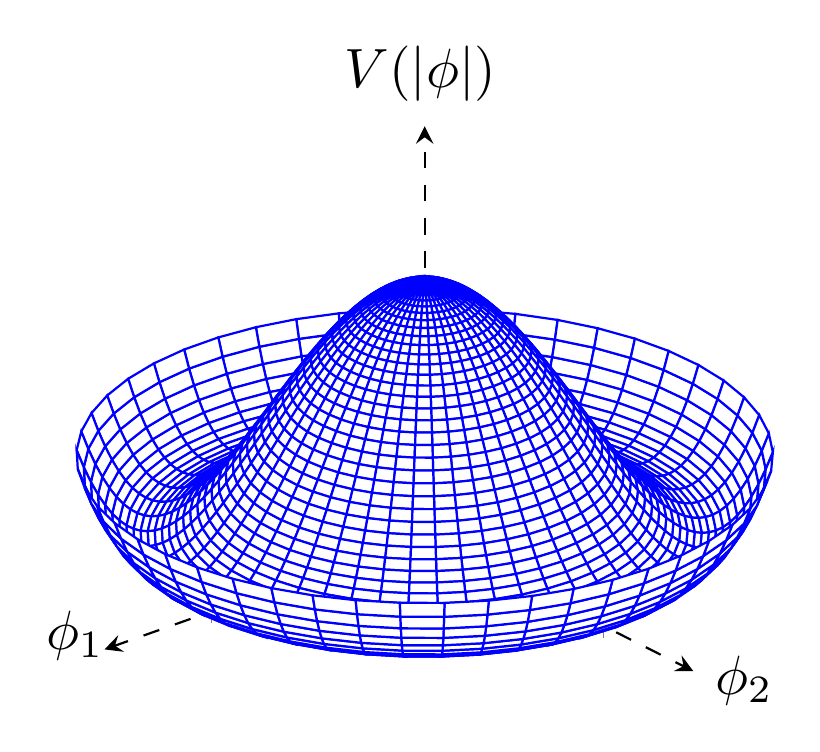
\begin{tikzpicture}[scale=2]
	\begin{axis}[
	axis lines = center,
	%axis on top = true,
	axis on top = false,
	axis line style = {black, thin, dashed},
	view = {140}{25},
	axis equal,
	colormap = {blackwhite}{gray(0cm)=(1); gray(1cm)=(0)},
	samples = 50,
	domain = 0:360,
	y domain = 0:1.25,
	zmin=0,
	xmax=1.5,
	ymax=1.5,
	zmax=1.5,
	yticklabels={,,},
	xticklabels={,,},
	zticklabels={,,},
	x label style={at={(axis description cs:0.18,0.25)},anchor=north},
	y label style={at={(axis description cs:0.8,0.2)},anchor=north},
	z label style={at={(axis description cs:0.5,0.88)},anchor=north},
	xlabel = $\phi_1$,
	ylabel=$\phi_2$,
	zlabel=$V(|\phi|)$
	]
	\addplot3 [surf, shader=flat, draw=blue, fill=white, z buffer=sort]
	   ({sin(x)*y}, {cos(x)*y}, {(y^2-1)^2});
	\end{axis}
\end{tikzpicture}
